\subsection{Spændingsforstærker}
\label{effekt_spaendingsforstaerker}
Spændingsforstærkerens opgave er at give en så stor spændingsforstærkning som muligt. Til dette projekts spændingsforstærker er der valgt en BC557B PNP-transistor koblet som en common-emitter. Koblingen af spændingsforstærkeren er vist på figur \ref{spaendingsforstaerker_diagram}

\begin{figure}[h]
\centering
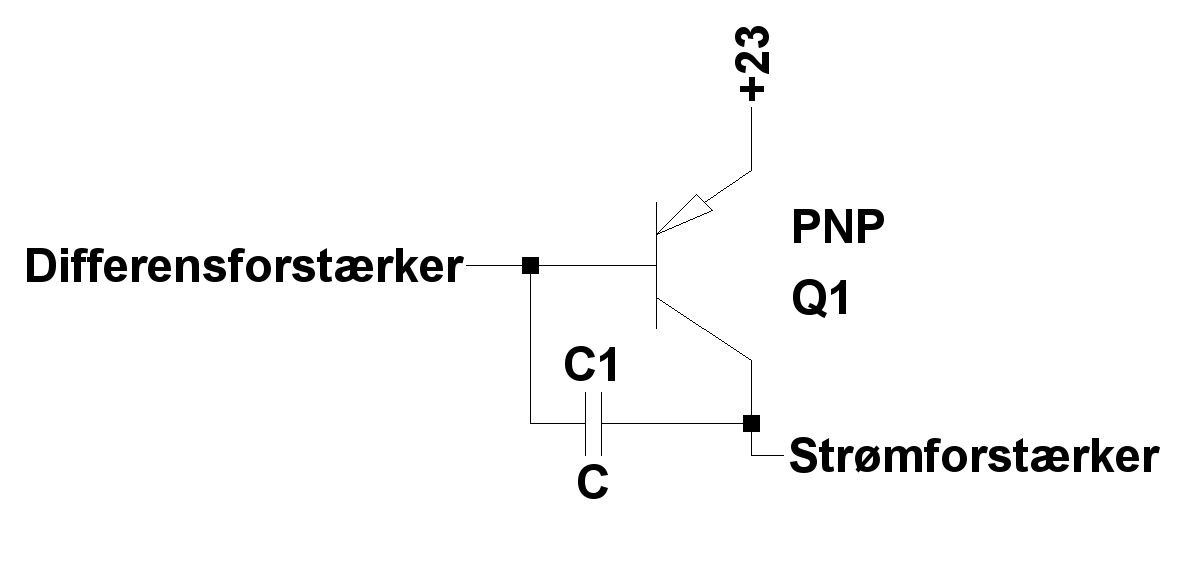
\includegraphics[scale=0.3]{teknisk/effektforstaerker/spaendingsforstaerker_diagram.png}
\caption{Diagram over opbygningen af spændingsforstærkeren.}
\label{spaendingsforstaerker_diagram}
\end{figure}

Forstærkningen i en commonemitter kobling er bestemt ved ligning (\ref{equ:spaendingsforstaerker1}) \cite{ael-mm7}%\fixme{Kilde: Jan analog elektronik mm7}
\begin{equation}
\label{equ:spaendingsforstaerker1}
A_v = -g_m \cdot || R'_L
\end{equation}

For at beregne $g_m$ bruges ligning (\ref{equ:spaendingsforstaerker2})\kilde{analog elektronik mm5}, hvor $I_c$ er den collectorstrøm som konstantstrømsgeneratoren trækker, og $V_T$ er sat til at være konstant $26~\mathrm{mV}$
\begin{equation}
\label{equ:spaendingsforstaerker2}
g_m = \frac{I_c}{V_T} = \frac{6~\mathrm{mA}}{26~\mathrm{mV}} = 230,8~\mathrm{mS}
\end{equation}

Modstanden $r_o$ kan beregnes ud fra ligning \ref{equ:spaendingsforstaerker50},  hvor $h_{\mathrm{oe}}$ og $h_{\mathrm{re}}$ er transistor parametre aflæst fra databladet.
\begin{equation}
\label{equ:spaendingsforstaerker50}
r_o = \frac{1}{h_{\mathrm{oe}} - g_m \cdot h_{\mathrm{re}}} = \frac{1}{60~\mathrm{\mu S} - 230,8~\mathrm{mS} \cdot 2 \cdot 10^{-4}} = 72,2~\mathrm{k}\ohm
\end{equation}

Nu skal $R'_L$ beregnes. $R'_L$ er defineret som den load spændingsforstærkeren ser. For at gøre det nemmere at beregne $R'_L$, er der lavet nogle antagelser. Første antagelse er at $V_\mathrm{be}$-multiplieren kan betragtes som en kortslutning, det kan gøres fordi $V_\mathrm{be}$-multiplieren fungere som et batteri der laver et DC-offset, mens AC potentialet  forbliver det samme på begge sider. Næste antagelse er at kortslutningskredsløbet kan ses bort fra, idet kredsløb ikke er aktuelt, når udgangen ikke er kortsluttet. Sidste antagelse er at den load $R'_L$ som spændingsforstærkeren ser er den ene af de to darlingtontransistorer i parallel med konstantstrømsgeneratoren. Dette fremkommer fordi der ses bort fra hvileområdet, hvor begge darlingtontrasistorer er aktive og kun ses på situationen, hvor der er fuld udstyring på en af transistorerne.
Med disse antagelser på plads kan impedansen $R'_L$ beregnes ud fra parallelkoblingen mellem konstantstrømsgeneratoren og en af darlingtontransistorerne.

Idet at konstantstrømsgeneratoren er en BC547B NPN-transistor koblet som en common-collector med uafkoblet emittermodstand, kan udgangsimpedansen beregnes ved ligning (\ref{equ:spaendingsforstaerker3})\fixme{Kilde: Analog elektronik mm7}
\begin{equation}
\label{equ:spaendingsforstaerker3}
R_{\mathrm{oc}} = r_o + R'_e + h_{\mathrm{fe}} \cdot r_o \cdot \frac{R'_e}{r_{\pi} + R_s || R_b}
\end{equation}

I ligning (\ref{equ:spaendingsforstaerker3}) er modstanden $R_s$ tilstede men i konstantstrømsgeneratoren er der ingen signalmodstand på basen. Modstanden $R'_e$ er 120 \ohm~og $r_o$ er givet ved ligning (\ref{equ:spaendingsforstaerker4}), hvor $h_{\mathrm{oe}}$ og $h_{\mathrm{re}}$ er transistor parametre aflæst fra databladet.
\begin{equation}
\label{equ:spaendingsforstaerker4}
r_o = \frac{1}{h_{\mathrm{oe}} - g_m \cdot h_{\mathrm{re}}} = \frac{1}{60~\mathrm{\mu S} - 230,8~\mathrm{mS} \cdot 2 \cdot 10^{-4}} = 72,2~\mathrm{k}\ohm
\end{equation}

Dernæst er potentialet fundet på basen af transistoren ved at tage den negative forsyning -23 V og trække de to diodespændingsfald fra og kortslutningsstrømmen er betsemt ved $\frac{23~\mathrm{V}}{2,7~\mathrm{k}\ohm}$ til 8,5 mA så derfor bliver $R_b = \frac{-21,56}{-8,5~mA} = 2,53~\mathrm{k}\ohm$. Modstanden $r_{\pi}$ er bestemt ved $\frac{h_{\mathrm{fe}}}{g_m} = \frac{330}{230,8~\mathrm{mS}} = 1,43~\mathrm{k}\ohm$. Den samlede impedans konstantstrømsgeneratoren repræsentere er beregnet i ligning (\ref{equ:spaendingsforstaerker5}). 
\begin{equation}
\label{equ:spaendingsforstaerker5}
R_{\mathrm{oc}} = 72,2~\mathrm{k}\ohm + 120~\ohm + 330 \cdot 72,2~\mathrm{k}\ohm \cdot \frac{120~\ohm}{1,43~\mathrm{k}\ohm + 2,7~\mathrm{k}\ohm} = 796~\mathrm{k}\ohm
\end{equation}


Darlingtontransistorerne der er valgt til projektet er opbygget som vist på figur \ref{darlington_diagram}. I databladet for darlingtontransistorerne \cite{bdx33-34-datablad} er R1 angivet til typisk at være 10 k\ohm~og R2 til 150 \ohm.

\begin{figure}[h]
\centering
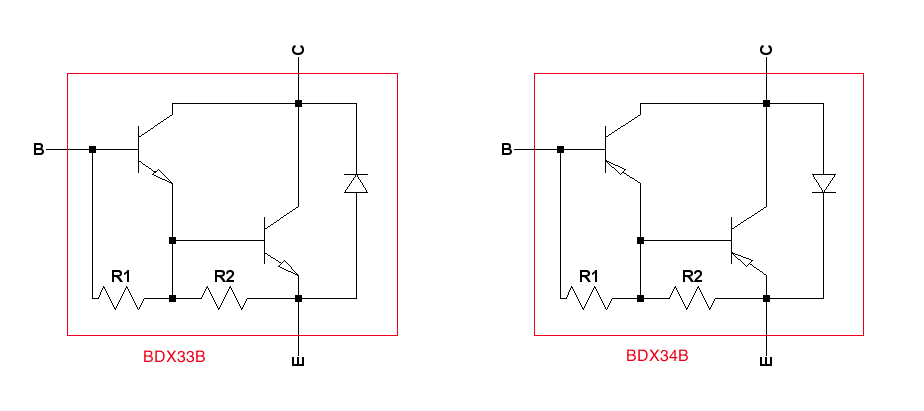
\includegraphics[scale = 0.4]{teknisk/effektforstaerker/darlingtontransistor_opbygning.png}
\caption{Diagram over opbygningen af darlingtontransistor BDX33B og BDX34B}
\label{darlington_diagram}
\end{figure}

For at gøre det nemmere at bestemme impedansen af darlingtontransistoren er det valgt at opfatte den som en enkelt supertransistor hvor $h_{\mathrm{fe}}= h_{\mathrm{fe}_1} \cdot h_{\mathrm{fe}_2}$ \cite{sedra-smith}. %\fixme{Kilde: sedra/smidth sixth edition side 525}
Der er også valgt at se bort fra de indre modstande i darlingtontransistoren. Når dette er valgt kan darlingtontransistoren i dette tilfælde opfattes som en transistor koblet som en commom-collector. Ud fra det kan der opstilles en simpel hybrid-$\pi$-model for supertransistoren som er vist i figur \ref{hybridpimodel_darlington}. Ud fra figur \ref{hybridpimodel_darlington} kan ligning (\ref{equ:spaendingsforstaerker6}) opsættes.

\begin{figure}[h]
\centering
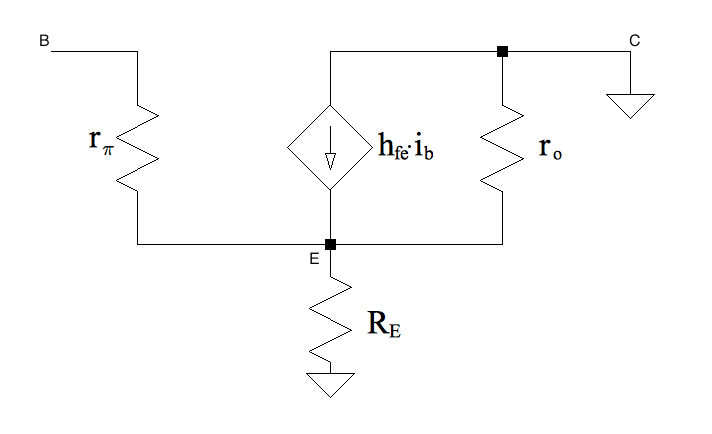
\includegraphics[scale=0.3]{teknisk/effektforstaerker/hybridpimodel.png}
\caption{Simpel småsignals hybrid-$\pi$-model  opstillet for supertransistor.}
\label{hybridpimodel_darlington}
\end{figure}
\begin{equation}
\label{equ:spaendingsforstaerker6}
v_b = i_b (r_{\pi} + (1+h_{\mathrm{fe}}) \cdot r_o||R_E) 
\end{equation}

Ligning (\ref{equ:spaendingsforstaerker3}) kan ved at dividere med $i_b$ på begge sider omskrives så det er indgangsimpedansen der regnes, dette er opstillet i ligning (\ref{equ:spaendingsforstaerker7})
\begin{equation}
\label{equ:spaendingsforstaerker7}
R_{\mathrm{in}} = r_{\pi} + (1+h_{\mathrm{fe}}) \cdot r_o||R_E 
\end{equation}

Fra databladet over darlingtontransistoren er $h_{\mathrm{fe}}$ angivet til minimum at være 750.  $R_E$ er den impedans der sidder efter darlingtontransistoren, som i dette tilfælde er en serieforbindelse af $R_e + R_L$, hvor $R_e$ er den termiske modstand og $R_L$ er den load højtaleren repræsentere. Transistorparameteren $r_{\pi}$ er givet ved $\frac{h_{\mathrm{fe}}}{g_m}$. Herefter opsættes Ligning (\ref{equ:spaendingsforstaerker9}) for at beregne indgangsimpedansen af darlingtontransistoren.
\begin{equation}
\label{equ:spaendingsforstaerker9}
R_{\mathrm{in}} = \frac{750}{230,8~\mathrm{mS}} + ( 1 + 750 ) \cdot 72,2~\mathrm{k}\ohm || (0,62~\ohm + 8~\ohm) = 9,77~\mathrm{k}\ohm  
\end{equation}

I ligning (\ref{equ:spaendingsforstaerker7}) får vi indgangsimpedansen for en darlingtontransistor til at være 9,77 k\ohm~og i ligning (\ref{equ:spaendingsforstaerker5}) får vi konstantstrømsgeneratoren impedans til $796~\mathrm{k}\ohm$. Derfor er den samledes impedans spændingsforstærkeren ser givet ved ligning (\ref{equ:spaendingsforstaerker10})
\begin{equation}
\label{equ:spaendingsforstaerker10}
R'_L = R_{\mathrm{in}}||R_{\mathrm{const}} = 9,77~\mathrm{k}\ohm || 796~\mathrm{k}\ohm = 9,65~\mathrm{k}\ohm
\end{equation}  

Med $R'_L$ for spændingsforstærkeren fundet er forstærkningen udregnet i ligning (\ref{equ:spaendingsforstaerker11})
\begin{equation}
\label{equ:spaendingsforstaerker11}
A_v = -g_m \cdot r_o || R'_L = 230,8~\mathrm{mS} \cdot 9,65~\mathrm{k}\ohm || 72.2~\mathrm{k}\ohm = -1964,44
\end{equation}

Hermed er forstærkningen i spændingsforstærkeren beregnet til at være 1964,44 med et fasedrej på 180\degree .